
This chapter describes the application I developed to segment tumor lesions using deep learning methods. The following sections describe the methodology of the solution, the implementation details, the parameters used, and the evaluation of the solution in the segmentation task.



\section{Dataset and preprocessing description}


The LiTS dataset was used to develop the solution and evaluate it. This dataset is described in section \ref{sec:lits}. The three-dimensional scans were randomly divided into training and testing data in proportions of 70/30, respectively, translating into 91 scans for training and 40 for testing.

In order to increase the amount of data, the three-dimensional scans were used to produce two-dimensional images called scan slices. Only every second slice was used, which still generated 21198 and 8158 training and testing images, respectively. The resulting images were single-channel grayscale. They were converted to three-channel images in RGB format to include more information in the images while emphasizing those of the liver. The individual channels were obtained as follows:
\begin{enumerate}
    \item The original grayscale image was subjected to HU windowing with a window level equal to 60 and window width equal to 200.
    \item The original grayscale image was subjected to histogram equalization.
    \item The original grayscale image was subjected to HU windowing with a window level equal to 30 and window width equal to 150.

\end{enumerate}

The values used as windowing parameters were chosen to increase the segmentation accuracy as much as possible. Since evaluating the solution for a given parameter value is very time-consuming, the issue has not been exhausted, and further research could be undertaken. The effect of the described processing can be seen in the figure \ref{fig:preproc_effect}.

\begin{figure}%
    \centering
    \subfloat[\centering Scan slice in greyscale]{{\includegraphics[width=5cm]{rysunki/orignal.jpg} }}%
    \qquad
    \subfloat[\centering Scan slice in RGB scale]{{\includegraphics[width=5cm]{rysunki/volume-0_slice_0.jpg} }}%
    \caption{Comparison of scan slice before and after preprocessing}%
    \label{fig:preproc_effect}%
\end{figure}


The model described in the following section also normalize and resize to 128x128 each input image.
\section{Methodology}
\subsection{Model architecture}

The U-Net architecture with ResNet34 as the backbone was used as the model for segmentation. Three components can be distinguished, occurring in sequence, of which the network is composed:
\begin{enumerate}
    \item ResNet34 that acts as an encoder.
    \item Bottleneck consisting of a layer of BatchNorm, ReLu, and a layer of double convolution.
    \item Decoder consisting of blocks from the classic U-Net architecture.
\end{enumerate}

Corresponding blocks from components 1 and 3 are connected via skip connections according to the assumptions behind the u-net architecture described in the section \ref{ref:u-net}. In the case of Resnet34, transfer learning was applied, a model with pre-trained weights was used. The model takes as input a batch of 16 images of size 128x128 and returns the probability that each pixel belongs to one of three classes:
\begin{enumerate}
    \item Background
    \item Liver
    \item Liver Tumor
\end{enumerate}
The class with the highest probability is the one to which the pixel belongs according to the model. Figure \ref{rys:my_arch} is the architecture of the model used; this visualization was made for a different task of segmentation of the compound, so the dimensions of the input of each layer are different.
\begin{figure}[!h]
	\centering 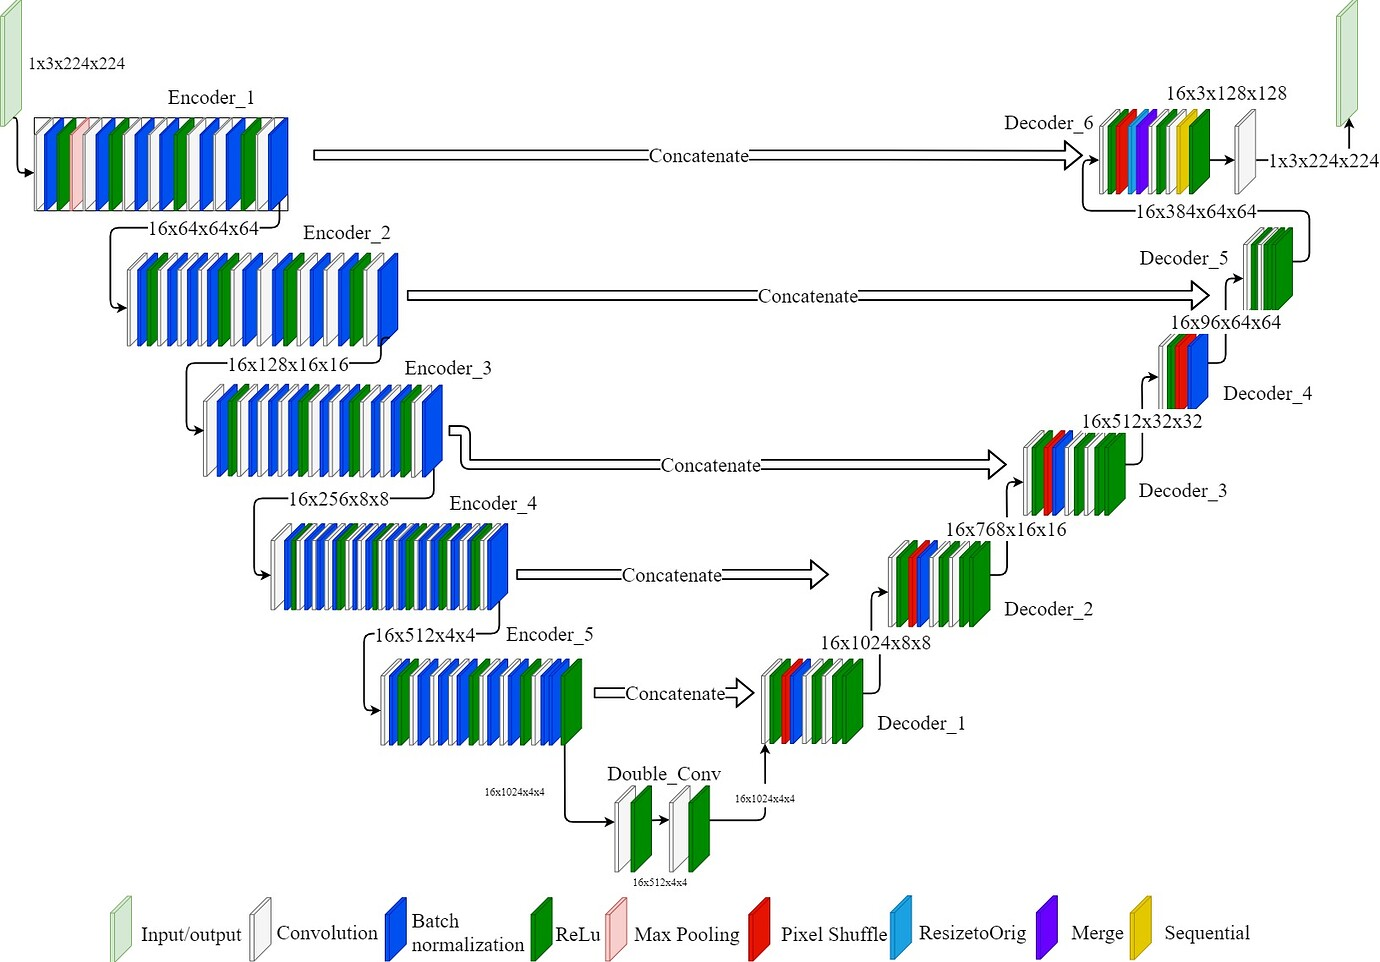
\includegraphics[width=\linewidth]{rysunki/135d5facd772ae16cee7360d0a0bbea8c74d5398_2_1380x962.jpeg}
	\caption{Architecture of network used in segmentation task. The image was created by user Adleman as part of discussion about this architecture on fastai framework forum \href{https://forums.fast.ai/t/u-net-with-resnet34-backbone/85744/4}{U-Net with ResNet34 backbone}.}
	\label{rys:my_arch}
\end{figure}

\subsection{Training Process}
As mentioned, the training has been conducted on a random subset representing $70\%$ of the total data. In addition, the data came to the model in batches of 16 images in size. An example of such a series can be seen in figure \ref{rys:batch}.

\begin{figure}[!h]
	\centering \includegraphics[width=\linewidth]{rysunki/another_batch.png}
	\caption{Example batch of training data. Segmentation masks have been overlaid on the input images, with red marking the liver and pink marking the tumor tissues.}
	\label{rys:batch}
\end{figure}
The hyperparameters used when training the network are listed in table \ref{tab:Hyperparameters}. For a larger number of epochs, the model did not significantly improve the operation, which is why this value was chosen. In the case of the loss function - its choice is arbitrary. However, exploring similar solutions on the Internet is one of the most common choices. In the case of learning rate, its value was chosen based on the LR range test described by Leslie Smith in \cite{smith_cyclical_2017}. This method selects the optimal learning rate based on going through one epoch of the model, changing the value of the learning rate during, and noting the corresponding value of the loss function. A randomly selected $20\%$ of the training data validates the model during training. For each epoch, the Dice coefficient achieved by the model in segmentation is also calculated.


 
\begin{table}[h!]
    \centering
    \begin{tabular}{|c|c|c|c|c|}
    \hline
        Hyperparameter & value  \\
        \hline 
        Number of epochs & 5 \\
        \hline
        Learning rate & 0.000091\\
        \hline
        Loss function & Cross-entropy\\
        \hline
    \end{tabular}
    \caption{Hyperparameters used for training networks }
    \label{tab:Hyperparameters}
\end{table}




\subsection{Testing}
A segmentation task was performed on a test data set to test the developed model. Based on the results, three evaluation metrics were used to examine how the model performed in variously defined tasks. The following metrics were used:
\begin{itemize}
    \item Dice coefficient
    \item Accuracy
    \item Precision
\end{itemize}
\label{model_testing}
These metrics were calculated for three different problems that the model is capable of solving:
\begin{enumerate}
    \item Segmentation of liver cancer lesions pixel-wise.
    \item Classification of whether a given input image shows a liver with cancer lesions.
    \item Classification of whether a patient has liver cancer lesions.
\end{enumerate}
The motivation for evaluating the model's performance in the context of problem number one is obvious. However, from the point of view of the practical applicability of such solutions, problems two and three are also significant. As mentioned in the introduction of this work, the reason for the high mortality rate of liver cancer is the problematic diagnosis of patients at an early stage of the disease. Gaining information about the existence of liver cancer tissues is, therefore, very valuable even if these lesions' segmentation is of low quality.
\section{Results}

\subsection{Training}

It took 4 hours and 36 minutes to train the model. The calculations took place on the CPU. The exact hardware specifications are described in the following section. The figure \ref{rys:plot_loss} shows the changing value of loss during training, both for the training and validation sets. In the figure \ref{rys:dice_training}, you can see the changing value of the Dice coefficient; this is a coefficient calculated for multi-class segmentation so that the segmentation efficiency of the liver itself is also included in this result. In figure \ref{rys:example_segs}, we can see the segmentation results performed on a specific random sample of data from the training data.



\begin{figure}[!h]
	\centering \includegraphics[width=0.7\linewidth]{rysunki/training_loss.png}
	\caption{Plot visualizing how values of training and validation loss changed during model training.}
	\label{rys:plot_loss}
\end{figure}

\begin{figure}[H]
	\centering \includegraphics[width=0.7\linewidth]{rysunki/dice_multi_class_training.png}
	\caption{Plot visualizing how value of Dice coefficient for multi-class segmentation changed during model training.}
	\label{rys:dice_training}
\end{figure}

\begin{figure}[H]
	\centering 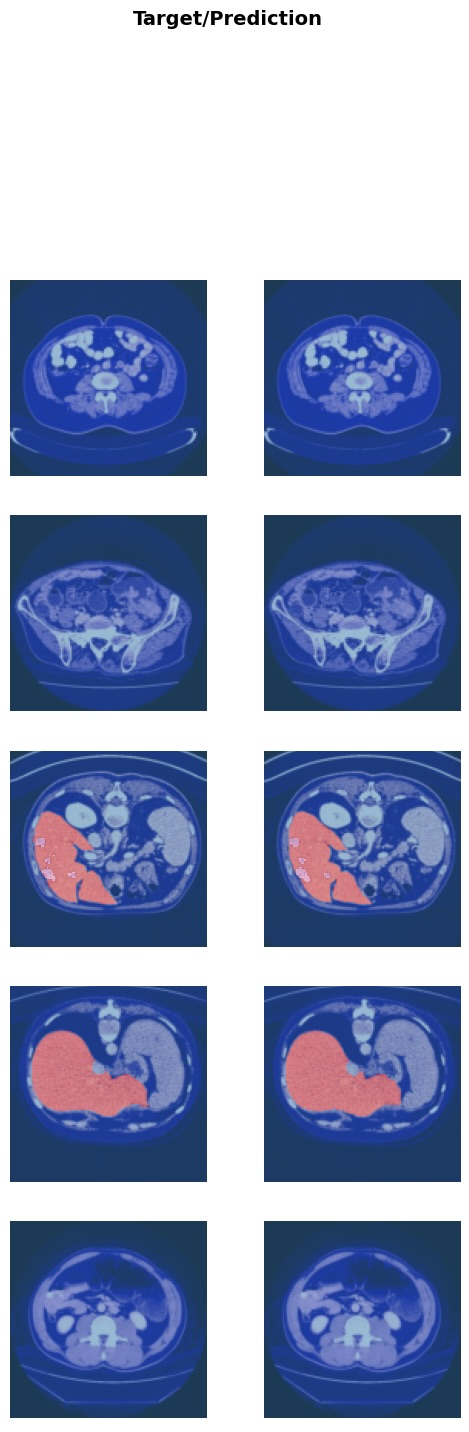
\includegraphics[scale=0.5]{rysunki/predykcje_modelu.jpeg}
	\caption{Segmentation performed on training set during model training. Red color marks the liver and pink tumor lesions}
	\label{rys:example_segs}
\end{figure}

\subsection{Testing}

It took about 0.5 seconds for the model to perform segmentation for one batch of test data. As described in the \ref{model_testing}, the same set of metrics was calculated for three different problems. The \ref{tab:metrics_prob_1} table presents the results that the model obtained in segmenting liver cancer lesions; these values refer to correctly classified pixels. In the \ref{tab:metrics_prob_2} table are presented the results that the model obtained in classifying a single input image as one with cancerous lesions. The \ref{tab:metrics_prob_3} table presents the results in classifying a patient with cancerous lesions. Figure \ref{fig:no_detected} shows an example of segmentation that did not detect existing tumor lesions. Instead, the figure \ref{fig:detected} shows a segmentation that detected existing lesions. Analysis of the results obtained is included in the next section.



\begin{table}[h!]
    \centering
    \begin{tabular}{|c|c|c|c|c|}
    \hline
        Metric & value  \\
        \hline 
        Accuracy & $0.99$ \\
        \hline
        Precision & $0.92$\\
        \hline
        Dice coefficient & $0.85$\\
        \hline
    \end{tabular}
    \caption{Evaluation metrics achieved by model in segmentation of cancer lesions.}
    \label{tab:metrics_prob_1}
\end{table}

\begin{table}[h!]
    \centering
    \begin{tabular}{|c|c|c|c|c|}
    \hline
        Metric & value  \\
        \hline 
        Accuracy & $0.95$ \\
        \hline
        Precision & $0.95$\\
        \hline
        Dice coefficient & $0.84$\\
        \hline
    \end{tabular}
    \caption{Evaluation metrics achieved by model in classifying single input image as one with cancerous lesions. }
    \label{tab:metrics_prob_2}
\end{table}

\begin{table}[h!]
    \centering
    \begin{tabular}{|c|c|c|c|c|}
    \hline
        Metric & value  \\
        \hline 
        Accuracy & $0.93$ \\
        \hline
        Precision &$0.95$ \\
        \hline
        Dice coefficient & $0.96$\\
        \hline
    \end{tabular}
    \caption{Evaluation metrics achieved by model in classifying classifying a patient with cancerous lesions.}
    \label{tab:metrics_prob_3}
\end{table}


\begin{figure}[H]%
    \centering
    \subfloat[\centering Ground truth mask over one of testing images]{{\includegraphics[width=5cm]{rysunki/prawidlowa_segmentacja1.png} }}%
    \qquad
    \subfloat[\centering Predicted mask over one of testing image]{{\includegraphics[width=5cm]{rysunki/segmentacja_model1.png} }}%
    \caption{Example of tumor lesions that were not detected by model. Green color represents liver and red one - tumor lesions.}%
    \label{fig:no_detected}%
\end{figure}



\begin{figure}[H]%
    \centering
    \subfloat[\centering Ground truth mask over one of testing images]{{\includegraphics[width=5cm]{rysunki/prawdilowa_segmentacja2.png} }}%
    \qquad
    \subfloat[\centering Predicted mask over one of testing image]{{\includegraphics[width=5cm]{rysunki/segmentacja_by_model2.png} }}%
    \caption{Example of tumor lesions that were detected by model. Green color represents liver and red one - tumor lesions.}%
    \label{fig:detected}%
\end{figure}

\section{Discussion}

The shape of the loss curves in the figure \ref{rys:plot_loss} may suggest that the so-called overfitting would occur if further training is done. Overfitting occurs when the model has learned to work too well with the training data and cannot generalize for new data. The possibility of overfitting is suggested by the fact that while the loss curve of the test set decreases all the time, the curve of the validation set decreases much more slowly, remaining at a certain stable level. The decrease in the rate of change and remaining stable is also evident in the graph with the value of the Dice coefficient on the test set during training in figure \ref{rys:dice_training}. Based on these two findings, it can be concluded that the number of epochs was chosen optimally; further training of the model would not improve its performance.

Most attention should be paid to the Dice coefficient for metrics evaluating the segmentation of liver cancer lesions in table \ref{tab:metrics_prob_1}. This is the most popular metric used by researchers, which makes it possible to compare the developed solution with solutions presenting the current state of knowledge in this issue. In such a comparison, the developed solution does not fare badly; the Dice coefficient obtained by it is $85\%$, and, as a review of current research in \ref{ref:state_of_art} shows, no model has yet been developed that the LiTS set would achieve a value equal to or greater than $90\%$. The uneven distribution of pixels can explain the very high accuracy value, most of which do not represent tumor tissue. Therefore, a very high number of TN (true negative pixels) may have distorted this particular metric. The high precision is a good indication of the model's performance; in this case, the results cannot be distorted since TN is not used in this metric. 

The model achieved similar results in classifying whether a given input image represents liver cancer; they can be seen in the table \ref{tab:metrics_prob_2}. The higher precision value shows even fewer misclassifications as an image representing cancerous lesions. The lower accuracy is due to the higher number of images with tumor lesions that went undetected. Nevertheless, it can still be considered very high.

The evaluative results of classifying a patient as having a cancerous lesion in table \ref{tab:metrics_prob_3} are satisfactory. The very high value of the Dice coefficient informs us of the low number of misclassifications. The accuracy is lower than those obtained for other problems. Despite the relevance of these results in applying a similar solution to the diagnosis of a broad group of people, it should be taken into account that they were obtained on a small number of patients (40), and the vast majority of them had cancerous lesions. If these results were achieved on a test set with a more significant number of patients, including those with healthy livers, it would prove that this type of solution has the potential to greatly facilitate the diagnosis of liver cancer at its early stage.




\section{Implementation and hardware details}

\subsection{Software and tools}

The application was implemented using the Python language version 3.11.4 \cite{python}. The following libraries were used in its development:
\begin{itemize}
    \item fastai  \cite{howard2018fastai} --- A deep learning library with high-level components that allow efficient and easy use of models that correspond to the current state of the art. The library uses the Pytorch framework \cite{NEURIPS2019_9015}  underneath.
    \item nibabel \cite{brett_2024_10714563} --- A library that allows reading data in NIfTi format, in which three-dimensional CT results are stored. With the library's help, it is possible to present this data in the form of a matrix.
    \item pandas \cite{reback2020pandas} -- A library that simplifies working with tabular data. 
    \item numpy \cite{harris2020array} --- A library that enables efficient numerical calculations on multidimensional arrays. In the project it is used to calculate evaluation metrics based on segmentation results.
\end{itemize}

\subsection{Modules}
The developed application consists of three Python modules:
\begin{itemize}
    \item data\_preprocessing.py --- This module contains the source data's logic for reading and preprocessing. The processed data is saved in folders for training or testing. 
    \item model\_training.py --- This module includes the logic for creating and training the model. The model uses train set created by previous module. Finally, the model is serialized and written to a file for reusability.
    \item model\_testing.py --- This module includes the logic for testing the model's performance on the test set. The trained model is read, and the corresponding metrics are calculated after the segmentation of the input data.

\end{itemize}
\subsection{Hardware details}
The experiments described in this chapter were conducted in the following computing environment:
\begin{itemize}
    \item Device name --- MacBook Air
    \item CPU and GPU --- Apple M1
    \item Ram memory -- 16 GB
\end{itemize}




